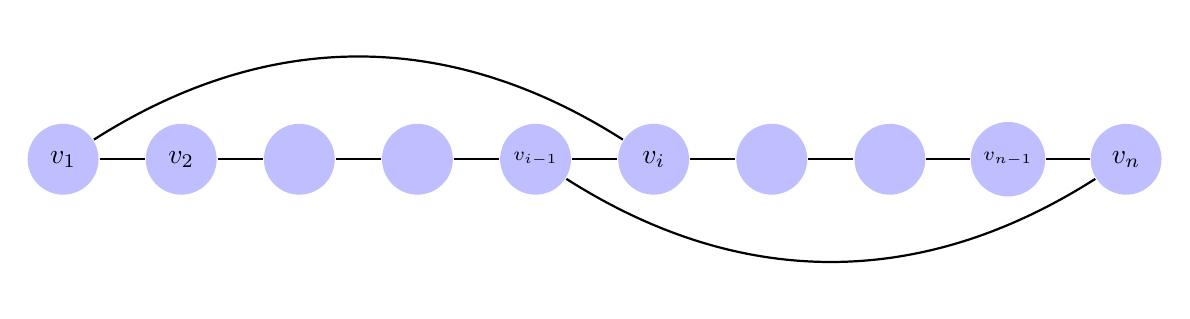
\begin{tikzpicture}                                         
[thick,auto,node distance=1.5cm,every node/.style={circle,minimum size=0.9cm,fill=blue!25}]
  \node (n1) {$v_1$};  
  \node (n2) [right of=n1] {$v_2$};
  \node (n3) [right of=n2] {};  
  \node (n4) [right of=n3] {};       
  \node (n5) [right of=n4] {\scriptsize $v_{i-1}$};
  \node (n6) [right of=n5] {$v_i$};
  \node (n7) [right of=n6] {}; 
  \node (n8) [right of=n7] {};         
  \node (n9) [right of=n8] {\scriptsize $v_{n-1}$};
  \node (n10) [right of=n9] {$v_n$};                                                
  \foreach \from/\to in {n1/n2,n2/n3,n3/n4,n4/n5,n5/n6,n6/n7,n7/n8,n8/n9,n9/n10}
    \draw (\from) -- (\to);
  \path                            
    (n1) edge [bend left=32.5] (n6)  
    (n10) edge [bend left=32.5] (n5);
\end{tikzpicture}
